\section{Remarkable Results and Conclusions}
A simulation performance metric without the inclusion of DA can be seen in Figures \ref{fig:06_hov_pena} and \ref{fig:06_bol_speedup} for experiments H1 and B1 respectively,
\begin{figure}[H]
	\centering
	\includegraphics[height=5.5cm,page=37,trim={10mm 15mm 20mm 35mm},clip]{Imagenes/06/hov/9u}%
	\includegraphics[height=5.5cm,page=37,trim={44mm 15mm 20mm 35mm},clip]{Imagenes/06/hov/9v}%
	\includegraphics[height=5.5cm,page=37,trim={44mm 15mm -20mm 35mm},clip]{Imagenes/06/hov/9vv}%
	\caption{Comparison of the H1 speed results (continuous line) vs. the simulation of Peña et. al. in 2013 (dotted line) and measured values (points). The data correspond to time averages between 12:00 and 15:00.}
	\label{fig:06_hov_pena}
\end{figure}
\begin{figure}[H]
	\centering
	\includegraphics[width=0.9\linewidth,trim={12mm 84mm -5mm 74mm},page=37,clip]{Imagenes/06/bol/speedup}\\%
	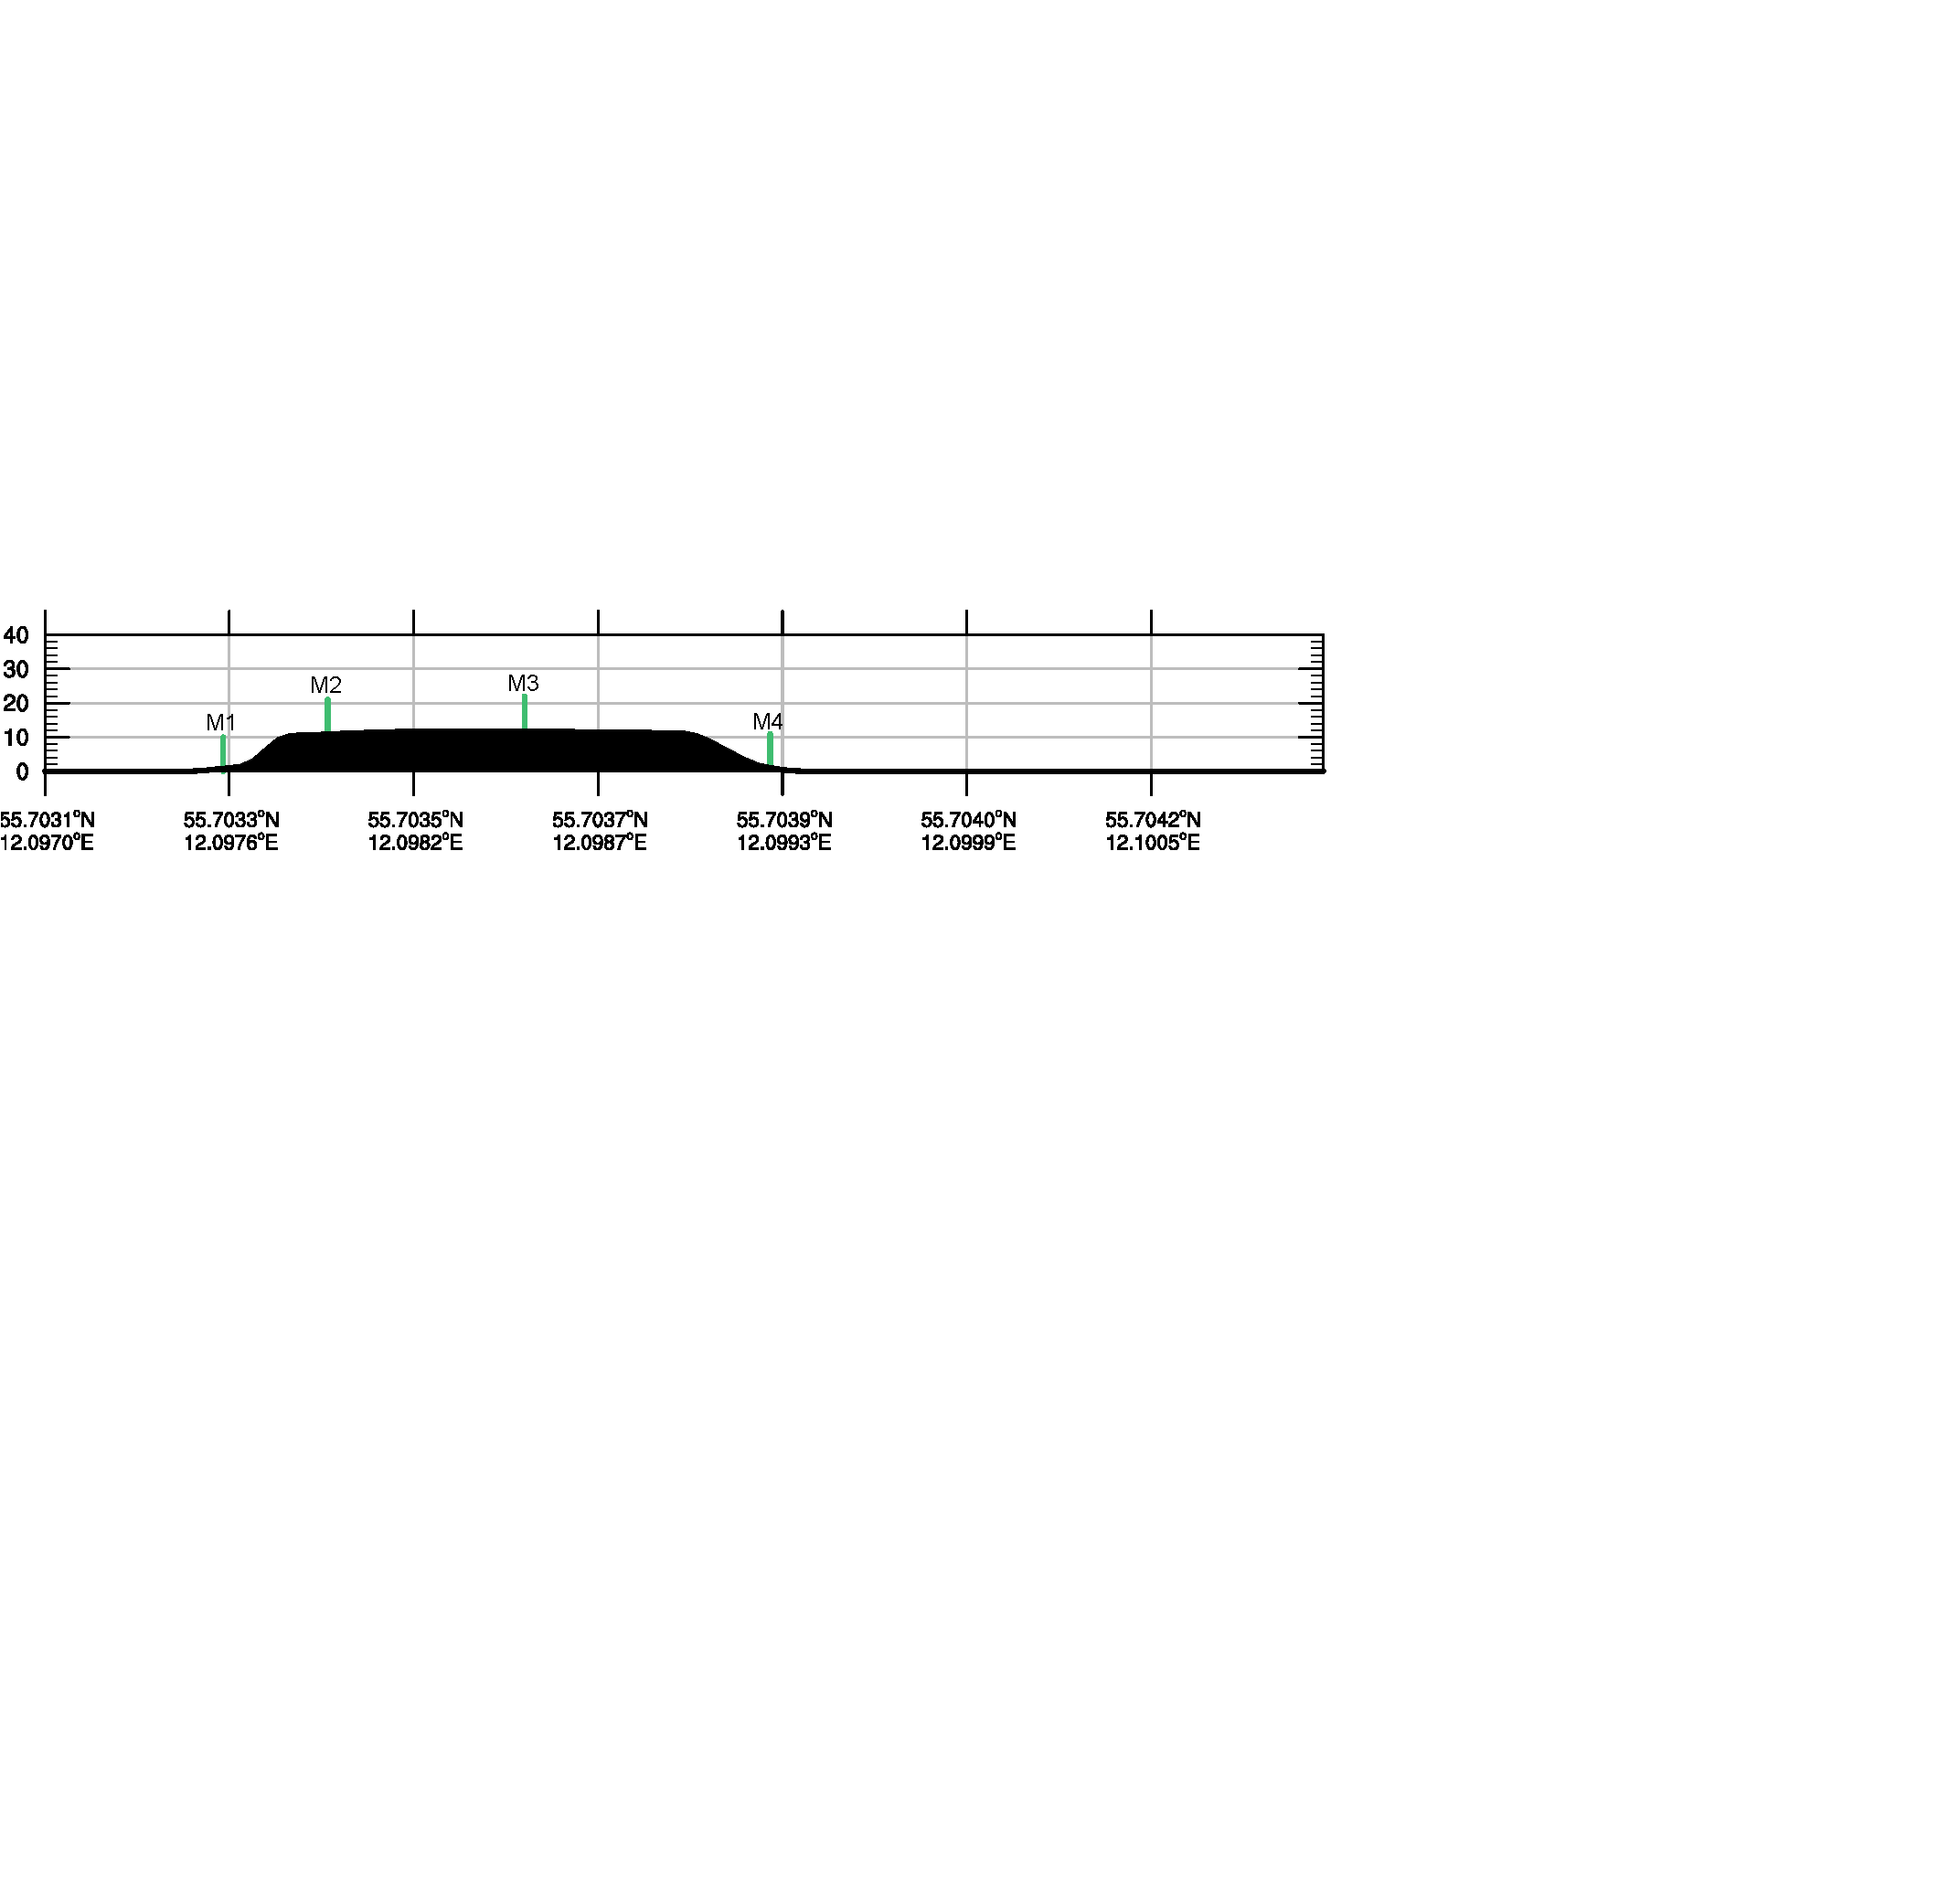
\includegraphics[width=0.9\linewidth,trim={-11mm 205mm 100mm 112mm},clip]{Imagenes/06/bol/cross_height}\\%
	\caption{Comparison of B1 speedup results at 15:00 vs. blind comparison. Values for the first 3 levels ($1.1$m blue; $3.4$m green; $5.6$m yellow) in section M1-M4 are shown.}
	\label{fig:06_bol_speedup}
\end{figure}
Here one can note that the high-resolution simulations met the expectations with respect to capturing: (i) the benchmark values for wind speed according to the validation cases and (ii) the qualitative behavior of the flow, both for flat terrain, as shown in Figure \ref{fig:05_dom_hov}, where the structures of the LES can be seen, and for complex terrain (Figure \ref{fig:05_mesh_bol}) where the streamlines expose the downstream boundary layer separation from the hill.

Regarding the performance of the DA, the Figures \ref{fig:06_hov_ts} and \ref{fig:06_bol_ts_m4} show the compared time series for a reference mast respectively. Note how in the first 6 hours of simulation (spinup) the data assimilation fixes the values to those measured.
\begin{figure}[H]
	\centering
	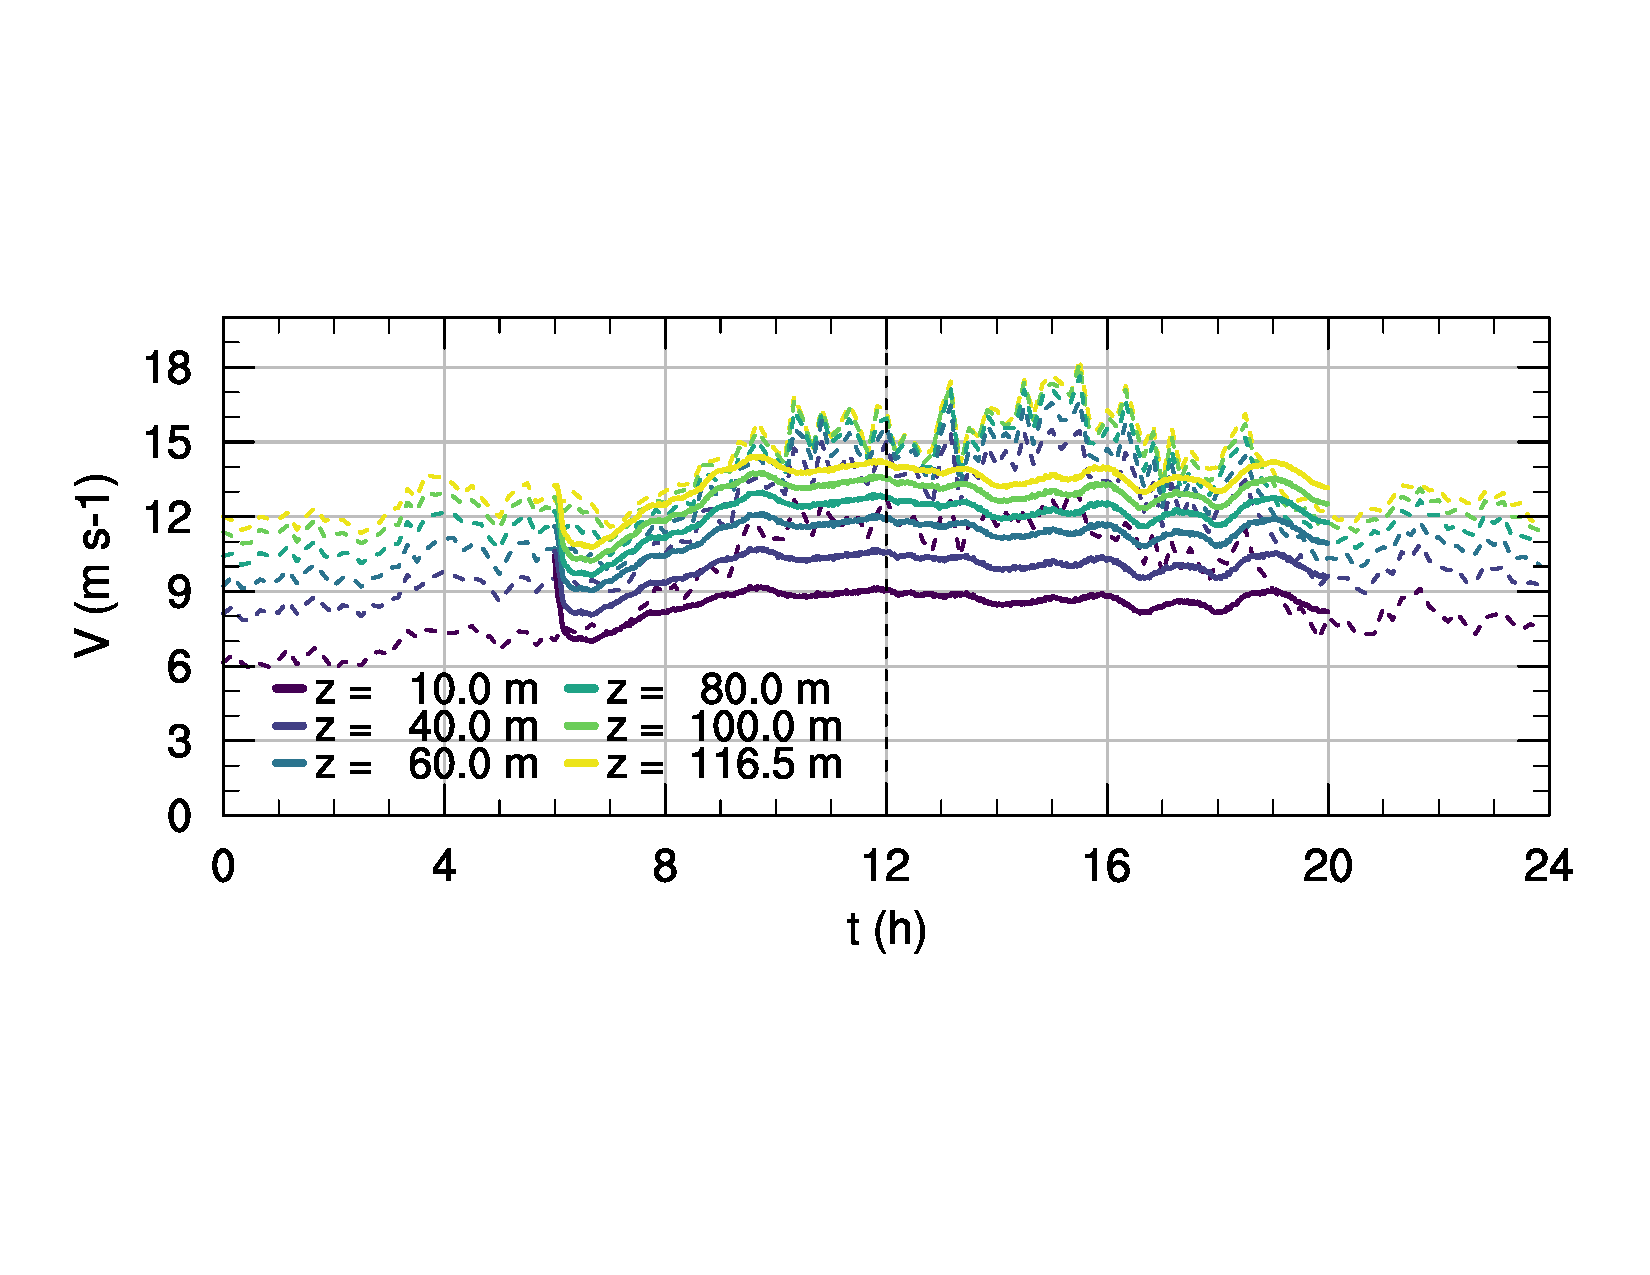
\includegraphics[width=0.5\linewidth,trim={7mm 75mm 10mm 50mm},clip]{Imagenes/06/hov/ts_v}%
	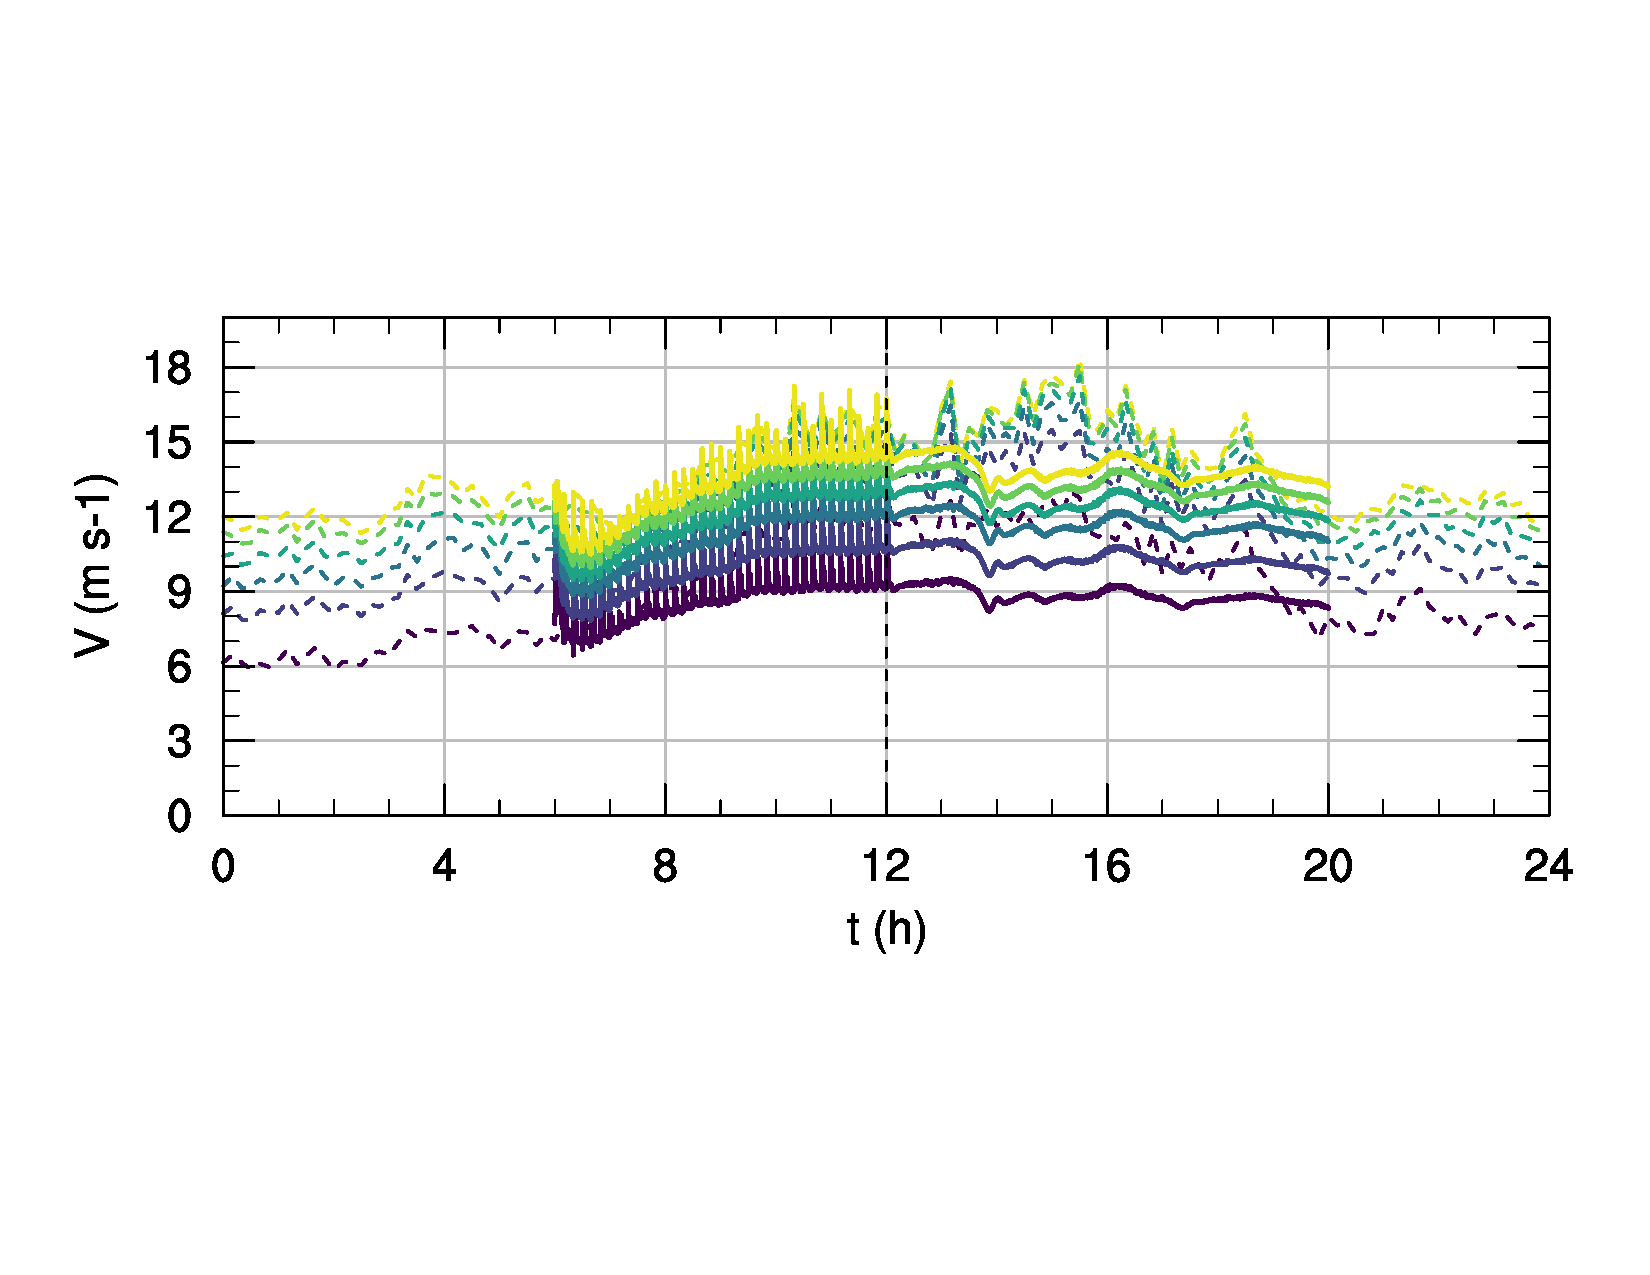
\includegraphics[width=0.5\linewidth,trim={35mm 75mm -18mm 50mm},clip]{Imagenes/06/hov_da/ts_v}%
	
	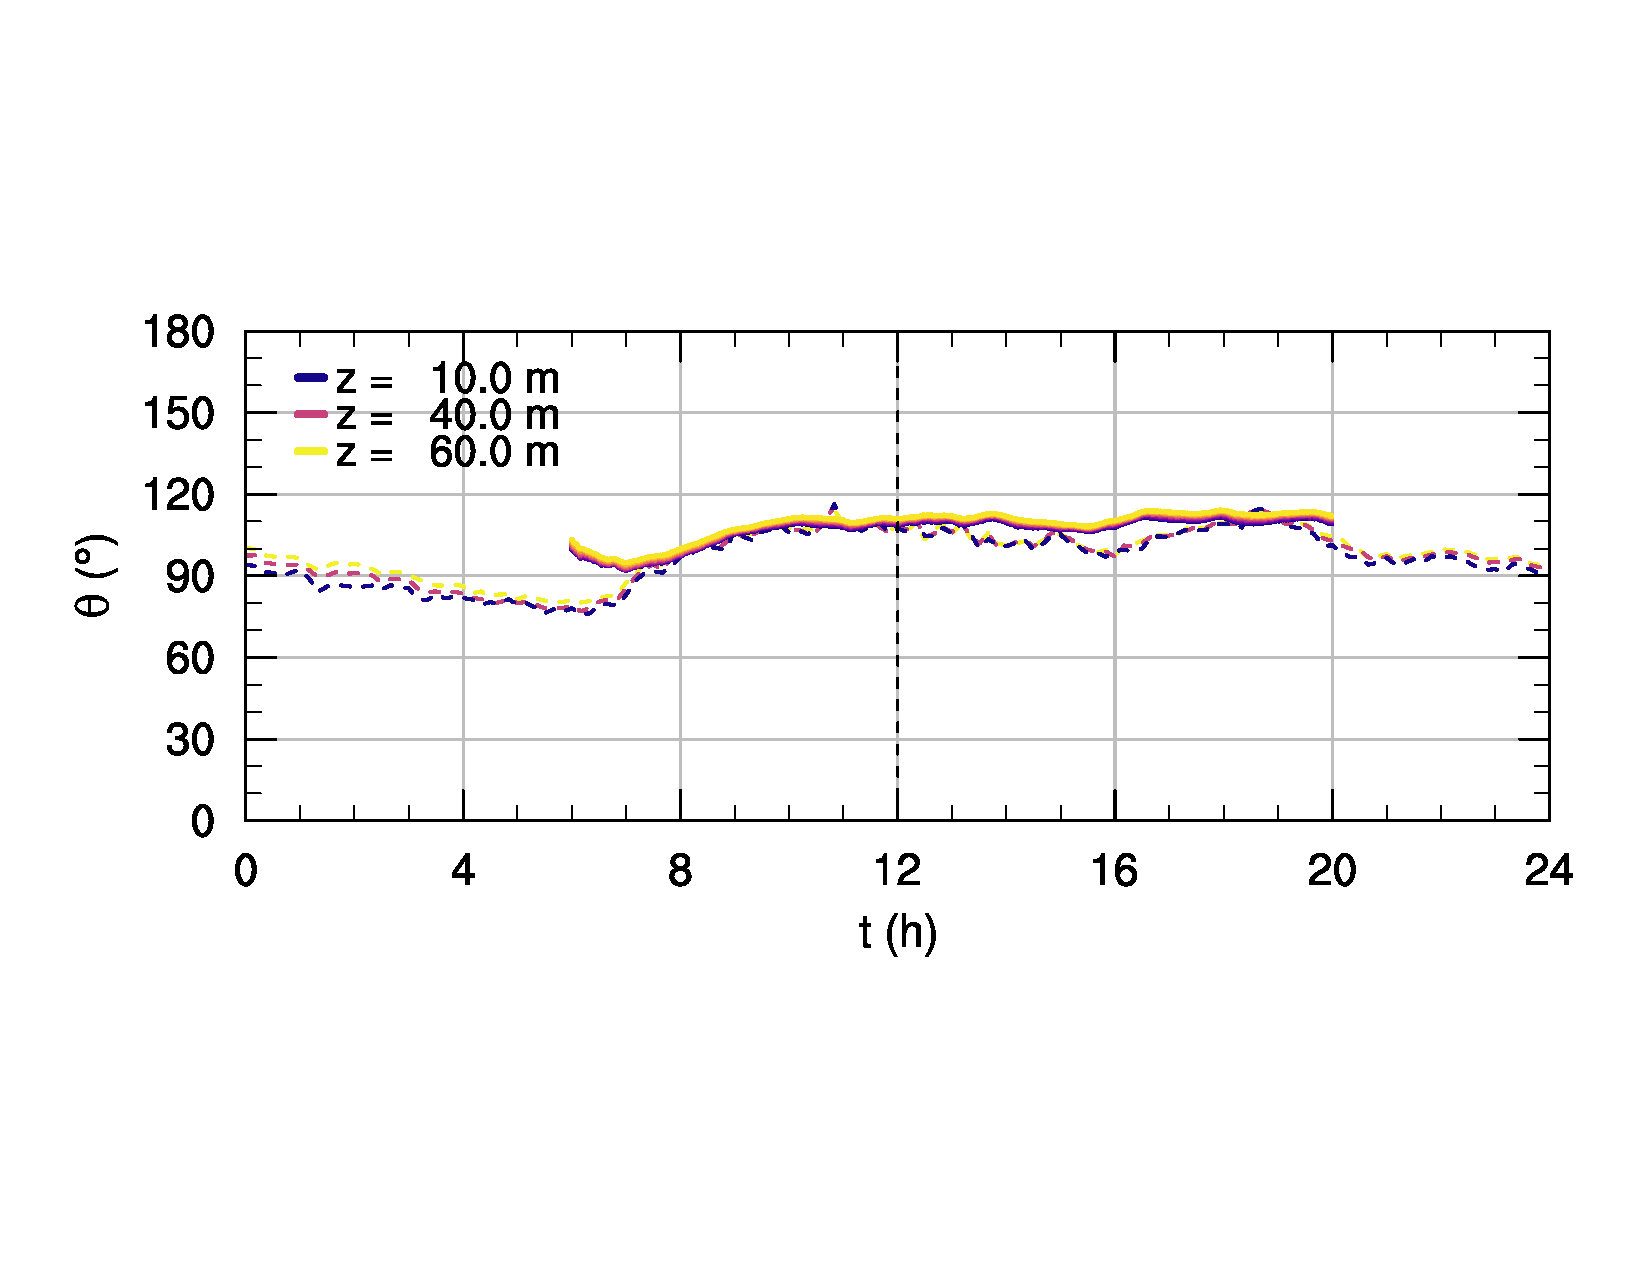
\includegraphics[width=0.5\linewidth,trim={12mm 53mm 10mm 50mm},clip]{Imagenes/06/hov/ts_o}%
	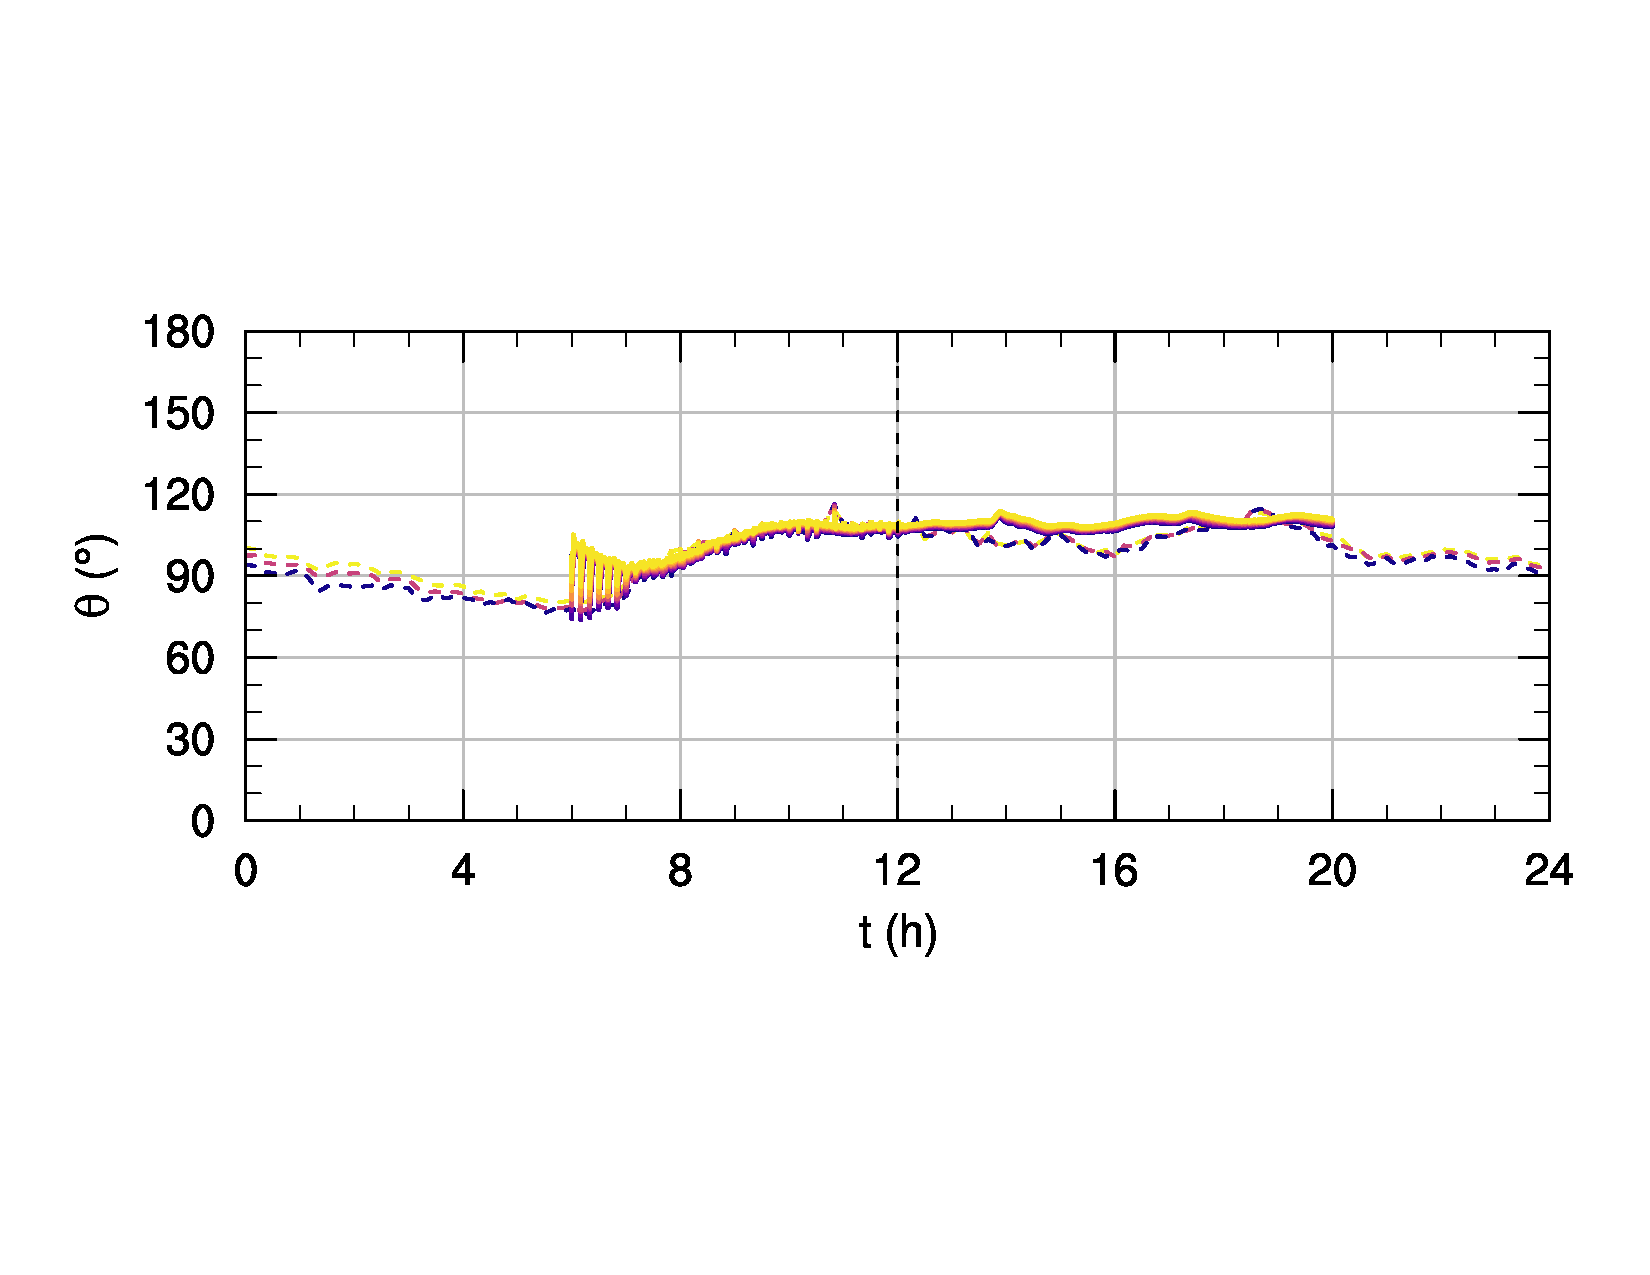
\includegraphics[width=0.5\linewidth,trim={38mm 53mm -16mm 50mm},clip]{Imagenes/06/hov_da/ts_o}%
	\caption{Time series for H1 vs. H2 at the met-mast. Simulation (solid line). Field data (dotted line)}
	\label{fig:06_hov_ts}
\end{figure}
\begin{figure}[H]
	\centering
	\includegraphics[width=0.5\linewidth,trim={7mm 68mm 10mm 55mm},page=3,clip]{Imagenes/06/bol/ts_interpol_compare.pdf}%
	\includegraphics[width=0.5\linewidth,trim={35mm 68mm -18mm 55mm},page=3,clip]{Imagenes/06/bol_da/ts_interpol_compare.pdf}%
	
	\includegraphics[width=0.5\linewidth,trim={12mm 48mm 10mm 55mm},page=3,clip]{Imagenes/06/bol/ts_interpol_compare_o.pdf}%
	\includegraphics[width=0.5\linewidth,trim={38mm 48mm -16mm 55mm},page=3,clip]{Imagenes/06/bol_da/ts_interpol_compare_o.pdf}%
	\caption{Time series for B1 vs. B2 at the M4 mast. Simulation (solid line). Field data (dotted line)}
	\label{fig:06_bol_ts_m4}
\end{figure}
Wind direction is broadly well represented in both simulations. The speed on the contrary acts differently in the two cases. For the H-experiments, there is a momentum deficit at low levels, possibly due to an overdiffusion in the LES. On the other hand, the simulation fails to capture the acceleration generated between 14:00 and 15:00 hours, and even though the application of DA allows to correct part of the deficit, it is still unsatisfactory for operational use. For B-experiments, the speed deficit in the low levels still exists, but in addition, it can be seen that the addition of DA negatively affects the performance of the simulation.
\begin{table}[H]
	\caption{Velocity metric comparison for all experiments in (m s-1)}
	\label{tab:06_bol_mae_rmse}
	\centering%\footnotesize
	\begin{tabular}{lcccc}
		\toprule
		& H1 & H2 & B1 & B2\\
		\midrule
		MAE& 2.41& 2.17 & 2.67 & 4.36 \\
		RMSE& 2.80& 2.56& 2.95& 4.90 \\
		\bottomrule
	\end{tabular}
\end{table}
The quantitative performance of the DA can be seen by using the defined metrics. Table \ref{tab:06_bol_mae_rmse} shows the summary for all cases. Here it can be seen that for the flat terrain case there is an improvement of about 10\% in the wind estimation, but for the complex terrain case the solution gets worse by almost 60\%. 


To conclude, it is relevant to highlight the following points:
\begin{itemize*}
\item It is possible to carry out microscale simulations through a mesoscale model that are satisfactory in both first order variables and wind behavior. The way to do this is by (i) using appropriate databases for terrain height and land use category and (ii) unifying the scales through an LES model. The simulated values for the H1 and B1 experiments show agreement with those presented in the literature using other types of methodologies.
\item Even though data assimilation proved improvements for the flat terrain case, the non-linearity of the complex terrain did not allow the DA to permeate to an improvement in the prediction of the wind resource. In addition to this, it is necessary to carry out more field experiments in order to have access to a larger amount of data in more masts and in this way to experiment with different data assimilation schemes for the improvement of simulations. In this work, data was assimilated within the boundary layer, stressing the associated turbulence model. One way to relax this is to assimilate data both inside and outside the boundary layer and in greater numbers across the domain.
\end{itemize*}







